\documentclass[11pt,a4paper]{article}

% --- 必要宏包加载 ---
\usepackage[utf8]{inputenc}
\usepackage[T1]{fontenc}
\usepackage{geometry}
\geometry{left=2.5cm,right=2.5cm,top=2.5cm,bottom=2.5cm}
\usepackage{booktabs} % 三线表核心：提供了不同粗细的横线
\usepackage{multirow} % 合并行
\usepackage{array}
\usepackage{amsmath}
\usepackage{float}    % 强制表格位置 [H]
\usepackage{graphicx} % 插入图片
\usepackage[font=small,labelfont=bf,labelsep=period]{caption}
\usepackage{subcaption} % 子图
\usepackage{hyperref}
% font=small: 标题字体变小
% labelfont=bf: "Table 1" 这种标签加粗
% labelsep=period: 标签后用句号分隔，更具学术感

\begin{document}

% --- 项目头部信息 ---
\begin{center}
    % 课程标题
    {\LARGE \textbf{CS5487 Course Project -- Group 98}} \\
\end{center}

% 个人信息块
\noindent
\rule{\linewidth}{0.8pt}\\
\textbf{Group ID:} 98 \\
\textbf{Topic:} (Default) Handwritten Digit Classification \\
\textbf{Group Members:} Zichun Cai (60080748), Wuyue Ma (59673599) \\
\rule{\linewidth}{0.8pt} % 底部的分割线
\vspace{1.5em}

\section{Introduction}
This project tackles \textbf{\textit{Handwritten Digit Classification}} on a subset of the \textbf{\textit{MNIST}} dataset, implemented in Python with \textbf{\textit{scikit-learn}}, \textbf{\textit{PyTorch}}, and the \textbf{\textit{XGBoost}} library.

Using \textbf{1-NN} as the baseline, we evaluate in-class methods — \textbf{\textit{Logistic Regression}} (linear) and \textbf{\textit{Kernel SVM}} (non-linear) — and extend to ensemble methods (\textbf{\textit{XGBoost}}, \textbf{\textit{Random Forest}}) and deep learning (\textbf{\textit{MLP}}, \textbf{\textit{CNN}}).

Results show the 1-NN baseline achieves 91.60\% while \textbf{CNN} reaches \textbf{98.10\%}, significantly outperforming all traditional models.

\section{Methodology}

\subsection{Classifier Selection}
We employ seven classifiers spanning four categories, summarized in Table~1.

\begin{table}[H]
    \centering
    \renewcommand{\arraystretch}{1.2} % 增加行高，视觉更舒适
    \small
    \begin{tabular}{lll}
        \toprule
        \textbf{Sub-category} & \textbf{Model Name} & \textbf{Key Characteristic} \\
        \midrule
        Baseline & 1-NN & Non-parametric, distance-based inference \\
        Linear & Logistic Regression & $L_2$ regularized probabilistic mapping \\
        Non-linear & Kernel SVM & RBF kernel for high-dimensional projection \\
        Ensemble & Random Forest & Bagging-based parallelized decision trees \\
        Ensemble & XGBoost & Iterative bias optimization via gradient boosting \\
        Neural Network & MLP & Dense connectivity for feature hierarchy \\
        Neural Network & CNN & Spatial inductive bias via convolutions \\
        \bottomrule
    \end{tabular}
    \caption{Taxonomy of implemented classification models.}
\end{table}

\subsection{Pre-processing Pipeline}
Raw 784-dimensional vectors are reshaped to $28 \times 28$ images, refined via \textbf{Median Filtering} and \textbf{Gaussian Smoothing}, then centered with \textbf{Centroid Centering}. The images are flattened, normalized to $[0, 1]$, and reduced with \textbf{PCA}.

\begin{table}[H]
    \centering
    \small
    \renewcommand{\arraystretch}{1.2} % 增加行高，视觉更舒适
    \begin{tabular}{clll}
        \toprule
        \textbf{Step} & \textbf{Operation} & \textbf{Setting} & \textbf{Purpose} \\
        \midrule
        1 & Reshape & $784 \to 28 \times 28$ & Restore spatial structure for filtering \\
        2 & Median Filter & $3 \times 3$ & Mitigate pixel-level noise \\
        3 & Gaussian Smoothing & $\sigma = 1.0$ & Reduce high-frequency noise \\
        4 & Centroid Centering & Shift to center & Standardize digit positioning \\
        5 & Flatten & $28 \times 28 \to 784$ & Revert to vector format \\
        6 & Min-Max Normalization & Scale to $[0, 1]$ & Ensure uniform feature contribution \\
        7 & PCA & Retain 95\% variance & Dimensionality reduction \\
        \bottomrule
    \end{tabular}
    \caption{Data preprocessing pipeline.}
\end{table}

\noindent \textbf{Model-Specific Adaptations:} \\
\textbf{1-NN} bypasses all preprocessing per course requirements. \textbf{XGBoost}, \textbf{Random Forest}, and \textbf{CNN} skip PCA, as these models handle high-dimensional input natively.

\section{Evaluation}

\subsection{Model Accuracy and Variance Analysis}
Each model is evaluated on two complementary trials (Trial~1: designated split; Trial~2: roles reversed). Table~\ref{tab:final_results} reports the results.

\begin{table}[H]
    \centering
    \renewcommand{\arraystretch}{1.3} % 优化行间距
    \small
    \begin{tabular}{lcccccc}
        \toprule
        \textbf{Models} & \textbf{Trial 1} & \textbf{Trial 2} & \textbf{Mean Acc.} & \textbf{Std.} & \textbf{F1-Score} & \textbf{Recall} \\
        \midrule
        \textbf{1-NN (Baseline)} & 0.9135 & 0.9185 & \textbf{0.9160} & 0.0025 & 0.9155 & 0.9160 \\
        \midrule
        Logistic Regression & 0.8890 & 0.8775 & 0.8832 & 0.0058 & 0.8827 & 0.8832 \\
        \textbf{Kernel SVM} & 0.9490 & 0.9470 & \textbf{0.9480} & 0.0010 & 0.9479 & 0.9480 \\
        XGBoost & 0.9200 & 0.9140 & 0.9170 & 0.0030 & 0.9168 & 0.9170 \\
        Random Forest & 0.9220 & 0.9155 & 0.9187 & 0.0033 & 0.9186 & 0.9187 \\
        MLP & 0.9425 & 0.9080 & 0.9253 & 0.0172 & 0.9251 & 0.9252 \\
        \textbf{CNN} & 0.9830 & 0.9790 & \textbf{0.9810} & 0.0020 & 0.9810 & 0.9810 \\
        \bottomrule
    \end{tabular}
    \caption{Experimental results of each algorithm.}
    \label{tab:final_results}
\end{table}

\noindent \textbf{\textit{Analysis:}}
\textbf{Kernel SVM} (94.80\%) leads traditional models with the lowest variance (0.0010), which is expected: the RBF kernel maps features into an infinite-dimensional space where digit classes become more separable, while the soft-margin objective ($C\!=\!10$) regularizes against overfitting. LR (88.32\%) falls below the 1-NN baseline because multinomial softmax can only learn linear decision boundaries in PCA space — insufficient for the complex topology of handwritten digits. The two ensemble methods, XGBoost (91.70\%) and RF (91.87\%), only marginally exceed 1-NN; this is likely because the PCA-reduced (or raw) feature space does not strongly favor tree-based splits over nearest-neighbor lookup at this scale. MLP (92.53\%) achieves moderate accuracy but exhibits the highest variance (0.0172), reflecting the sensitivity of gradient-based optimization to the random weight initialization and the particular train/test partition. \textbf{CNN} (98.10\%) is the clear winner: its convolutional layers exploit the 2D spatial structure of digit images — translation invariance and local feature hierarchies — giving it a fundamental advantage that flat-vector methods lack. On the base set, F1-Score and Recall closely track Accuracy for all models, indicating that the per-class performance is well-balanced and no single digit is systematically neglected.

\subsection{Challenge Dataset Performance}

We further test on the ``Challenge'' subset (Table~\ref{tab:challenge_results}).

\begin{table}[H]
    \centering
    \renewcommand{\arraystretch}{1.3}
    \small
    \begin{tabular}{lcccccc}
        \toprule
        \textbf{Models} & \textbf{Trial 1} & \textbf{Trial 2} & \textbf{Mean Acc.} & \textbf{Std.} & \textbf{F1-Score} & \textbf{Recall} \\
        \midrule
        \textbf{1-NN (Baseline)} & 0.6600 & 0.7067 & \textbf{0.6833} & 0.0233 & 0.6757 & 0.6833 \\
        \midrule
        Logistic Regression & 0.7533 & 0.7867 & 0.7700 & 0.0167 & 0.7644 & 0.7700 \\
        \textbf{Kernel SVM} & 0.8467 & 0.8667 & \textbf{0.8567} & 0.0100 & 0.8560 & 0.8567 \\
        XGBoost & 0.7667 & 0.8267 & 0.7967 & 0.0300 & 0.7960 & 0.7967 \\
        Random Forest & 0.7733 & 0.8133 & 0.7933 & 0.0200 & 0.7892 & 0.7933 \\
        MLP & 0.7867 & 0.8067 & 0.7967 & 0.0100 & 0.7946 & 0.7967 \\
        \textbf{CNN} & 0.9267 & 0.9200 & \textbf{0.9233} & 0.0033 & 0.9195 & 0.9233 \\
        \bottomrule
    \end{tabular}
    \caption{Experimental results on the Challenge dataset.}
    \label{tab:challenge_results}
\end{table}

\noindent \textbf{\textit{Analysis:}} All models degrade on the challenge set due to distribution shift — the challenge digits likely come from different writers with different stroke styles, violating the i.i.d.\ assumption. 1-NN drops most severely (91.60\% $\to$ 68.33\%) because nearest-neighbor classification relies on the training manifold being locally smooth; when test points lie in unfamiliar regions of pixel space, the nearest neighbor becomes meaningless. LR (77.00\%) now surpasses 1-NN: even a suboptimal learned boundary captures \emph{structural} patterns (stroke angles, curvature) that transfer across distributions, whereas raw $\ell_2$ distance does not. Kernel SVM holds at \textbf{85.67\%} thanks to the RBF kernel's ability to define flexible, data-adaptive boundaries. \textbf{CNN} remains best at \textbf{92.33\%}, losing only 6 points — its hierarchical feature extraction (edges $\to$ strokes $\to$ parts) learns representations that are inherently more invariant to style variations. F1-Score now diverges from Accuracy on weaker models (e.g., 1-NN: F1\,=\,0.6757 vs Acc\,=\,0.6833), confirming that the distribution shift affects certain digit classes (those with more style variability) disproportionately.

\subsection{Error Pattern Analysis}

To understand which digits are hardest, we examine per-class recall (Figure~\ref{fig:error_analysis}) and top misclassification pairs.

\begin{figure}[H]
    \centering
    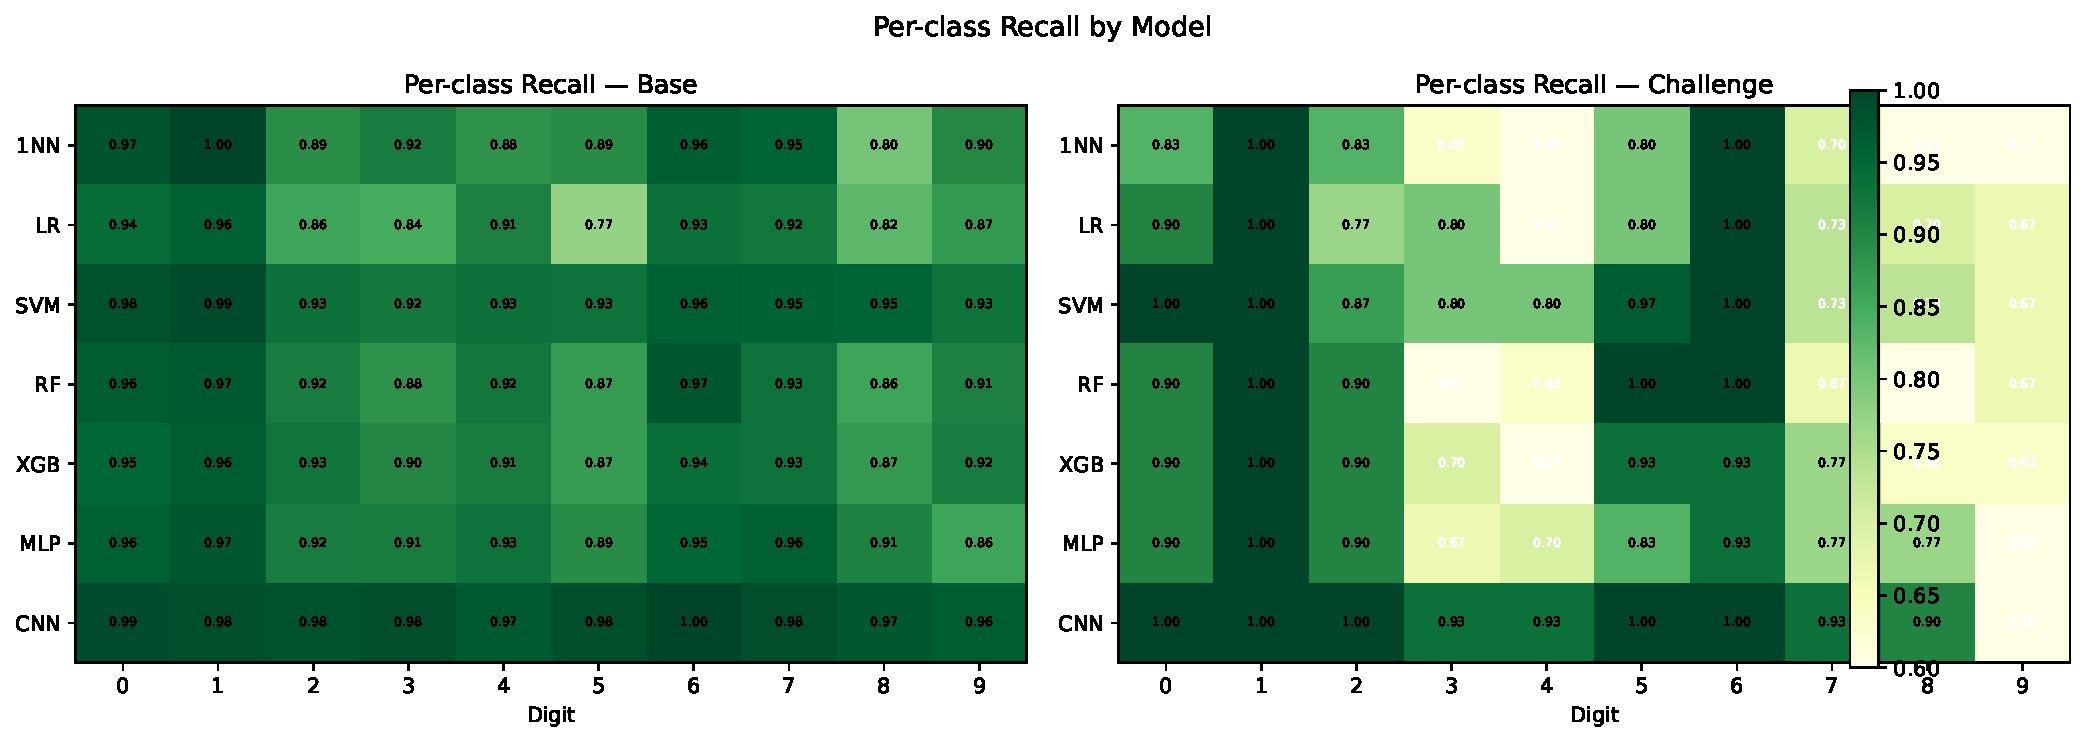
\includegraphics[width=\textwidth]{results/eval_figures/eval_error_analysis.pdf}
    \caption{Per-class recall heatmap for all models on base (left) and challenge (right) datasets.}
    \label{fig:error_analysis}
\end{figure}

\noindent \textbf{\textit{Analysis:}} On the base set, the dominant error is \textbf{4$\to$9} (34 times for 1-NN). This is expected: handwritten 4 and 9 share a closed upper loop, making them difficult to distinguish by pixel-level or even low-level features. The cluster \textbf{3, 5, 8} also shows mutual confusion due to overlapping curved strokes — all three digits consist primarily of arcs and loops that produce similar feature vectors after PCA projection. LR struggles especially with \textbf{3$\leftrightarrow$5} because a linear hyperplane in PCA space cannot capture the subtle curvature differences that distinguish these two digits. On the challenge set, \textbf{9$\to$1} and \textbf{4$\to$1} emerge as dominant errors for 1-NN, suggesting that the challenge data contains thinner, more elongated strokes: when a 4 or 9 is written with a single vertical stroke, its pixel representation becomes indistinguishable from 1 under $\ell_2$ distance. CNN's remaining errors concentrate on the inherently ambiguous \textbf{4$\leftrightarrow$9} and \textbf{9$\to$7} pairs — even with learned hierarchical features, these digit pairs overlap near the decision boundary, representing the practical limit of visual discriminability on this dataset.

\subsection{Hyperparameter Sensitivity Analysis}

Exhaustive grid searches are impractical with our from-scratch code. We first quantify the speed gap, then use \textit{sklearn} for the sweeps.

\subsubsection{From-Scratch vs Library Speed Comparison}
\label{sec:speed}

All benchmarks are performed under the environment listed in Table~\ref{tab:env}.

\begin{table}[H]
    \centering
    \renewcommand{\arraystretch}{1.15}
    \small
    \begin{tabular}{ll}
        \toprule
        \textbf{Component} & \textbf{Specification} \\
        \midrule
        CPU   & Intel Core i9-14900 (24 cores) \\
        RAM   & 64\,GB DDR5 \\
        GPU   & NVIDIA RTX A1000 (used only for CNN) \\
        OS    & Ubuntu 24.04 LTS \\
        Python & 3.12 \\
        \bottomrule
    \end{tabular}
    \caption{Hardware and software environment.}
    \label{tab:env}
\end{table}

\noindent Table~\ref{tab:speed} and Figure~\ref{fig:speed} compare training time on Trial~1 under identical preprocessing.

\begin{table}[H]
    \centering
    \renewcommand{\arraystretch}{1.2}
    \small
    \begin{tabular}{llccc}
        \toprule
        \textbf{Component} & \textbf{Implementation} & \textbf{Acc.} & \textbf{Time (s)} & \textbf{Ratio} \\
        \midrule
        \multirow{2}{*}{PCA}
            & From-scratch (\texttt{eigh})  & —      & 0.07  & \multirow{2}{*}{0.2$\times$ (faster)} \\
            & \textit{sklearn} PCA          & —      & 0.33  & \\
        \midrule
        \multirow{2}{*}{Logistic Regression}
            & From-scratch (L-BFGS-B)       & 0.8810 & 0.16  & \multirow{2}{*}{9$\times$ slower} \\
            & \textit{sklearn} LR           & 0.8805 & 0.02  & \\
        \midrule
        \multirow{2}{*}{Kernel SVM}
            & From-scratch (SMO, OvR)       & 0.9490 & 15.1  & \multirow{2}{*}{145$\times$ slower} \\
            & \textit{sklearn} SVC          & 0.9415 & 0.10  & \\
        \midrule
        \multirow{2}{*}{Random Forest}
            & From-scratch                  & 0.9155 & 16.3  & \multirow{2}{*}{86$\times$ slower} \\
            & \textit{sklearn} RF           & 0.9133 & 0.19  & \\
        \bottomrule
    \end{tabular}
    \caption{From-scratch vs \textit{sklearn} training speed on Trial~1.}
    \label{tab:speed}
\end{table}

\begin{figure}[H]
    \centering
    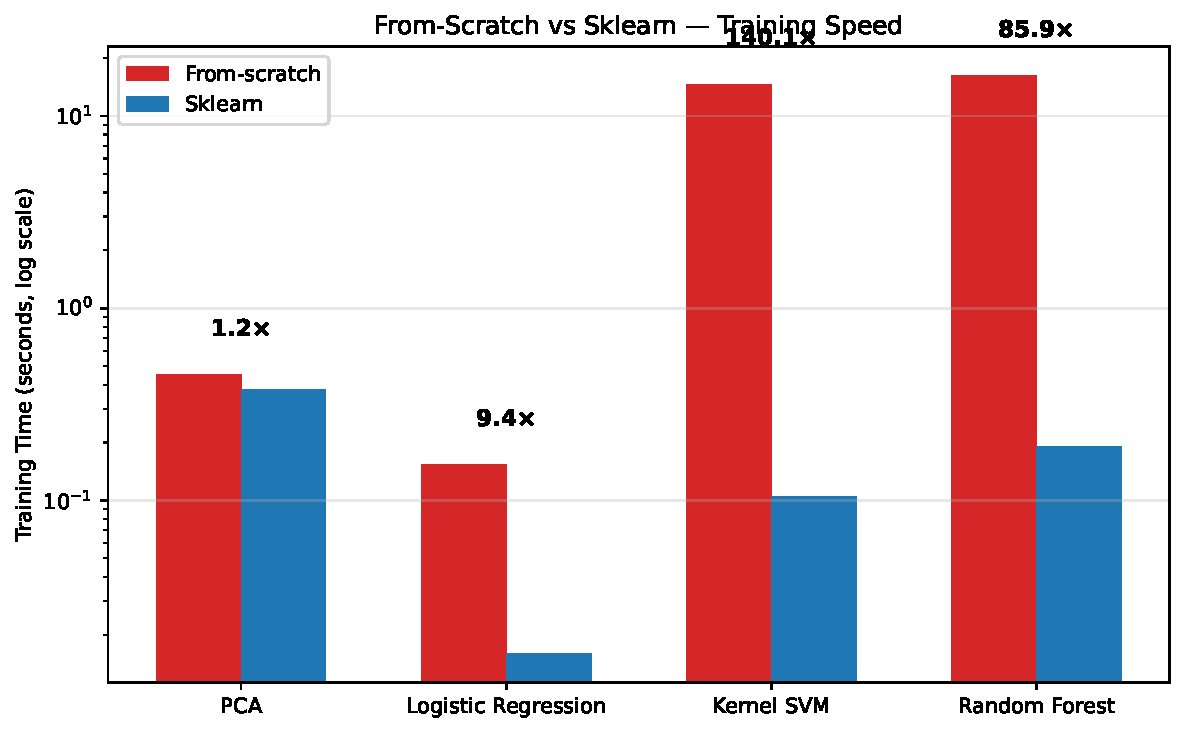
\includegraphics[width=0.82\textwidth]{results/eval_figures/eval_speed_comparison.pdf}
    \caption{From-scratch vs Sklearn — training time comparison (log scale).}
    \label{fig:speed}
\end{figure}

\noindent \textbf{\textit{Analysis:}} Our from-scratch PCA is actually faster (0.07\,s vs 0.33\,s) because it directly calls \texttt{numpy.linalg.eigh} on the covariance matrix, whereas sklearn's \texttt{PCA} includes additional overhead for input validation, automatic solver selection, and numerical stability checks. For classifiers, the gap reverses dramatically: LR is 9$\times$ slower, RF 86$\times$, and SVM 145$\times$ slower. The SVM gap is the largest because our simplified SMO algorithm performs $O(n^2)$ kernel evaluations per pass in interpreted Python, whereas sklearn's \texttt{libsvm} backend is written in optimized C with efficient kernel caching and shrinking heuristics. Similarly, our RF builds trees with Python-level loops over feature splits, while sklearn uses parallelized Cython code. Despite the speed disadvantage, our from-scratch SVM achieves \emph{higher} accuracy (94.90\% vs 94.15\%), likely because the SMO convergence criteria differ — our implementation runs more passes, effectively performing more thorough optimization. Given that a single SVM grid search over 35 $(C, \gamma)$ combinations would require $35 \times 15\text{s} \approx 9$ minutes with our code versus $\sim$4\,s with sklearn, all subsequent hyperparameter sweeps use sklearn.

\subsubsection{SVM Kernel Comparison}
The kernel determines the feature space for SVM's separating hyperplane. We sweep $C \in \{10^{-3}, \ldots, 10^{3}\}$ across five kernels (Linear, RBF, Poly, Sigmoid).

\begin{figure}[H]
    \centering
    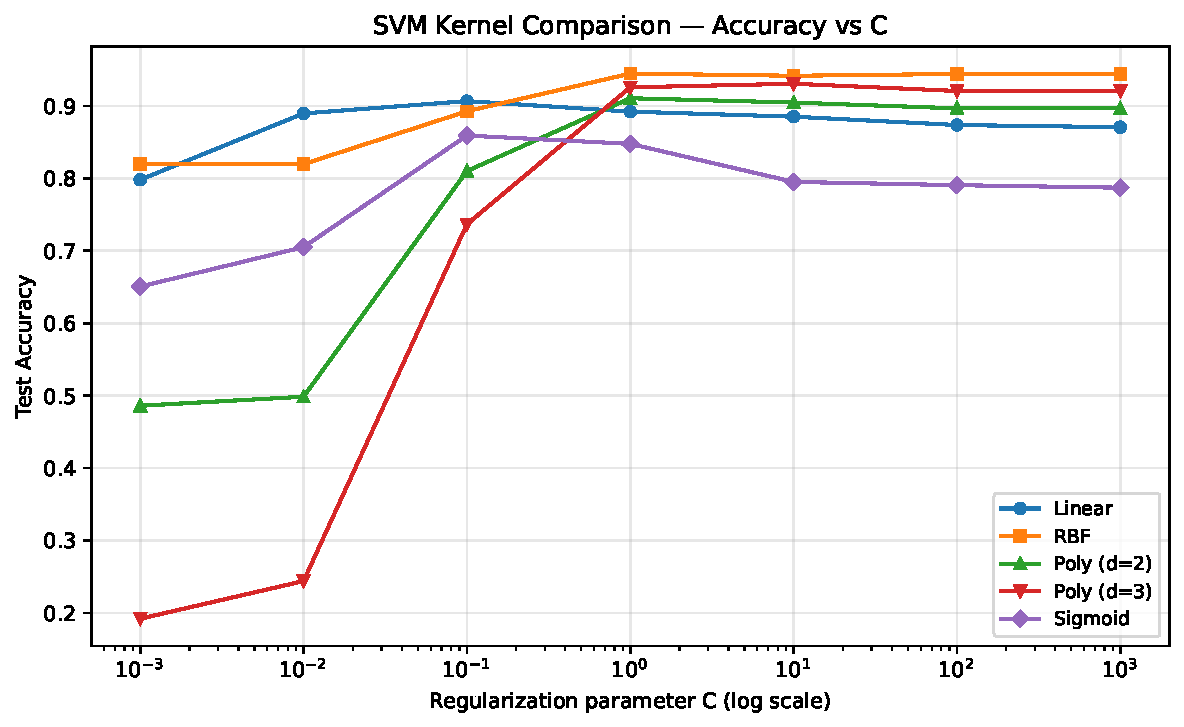
\includegraphics[width=0.85\textwidth]{results/eval_figures/eval_svm_kernel.pdf}
    \caption{SVM kernel comparison — test accuracy as a function of $C$ on Trial~1.}
    \label{fig:svm_kernel}
\end{figure}

\noindent \textbf{\textit{Analysis:}} The \textbf{RBF kernel} dominates for $C \geq 1$ ($\approx$94.4\%), which is theoretically expected: RBF maps input features into an infinite-dimensional Hilbert space via $K(\mathbf{x},\mathbf{x}') = \exp(-\gamma \|\mathbf{x}-\mathbf{x}'\|^2)$, enabling the SVM to construct highly non-linear decision boundaries. The Linear kernel peaks at $C\!=\!0.1$ (90.7\%) then degrades with larger $C$ — increasing $C$ forces the linear model to fit training noise, confirming that the 10-class digit boundaries in 32-dimensional PCA space are intrinsically non-linear. Polynomial kernels ($d\!=\!2,3$) approach RBF at high $C$ but exhibit less stable convergence. Sigmoid performs poorly throughout, consistent with its known theoretical issues (it does not always yield a valid positive semi-definite kernel matrix).

\subsubsection{SVM Grid Search Visualization}
For RBF, $C$ controls the bias-variance trade-off and $\gamma$ controls kernel width. We search $(C, \gamma)$ with 5-fold CV.

\begin{figure}[H]
    \centering
    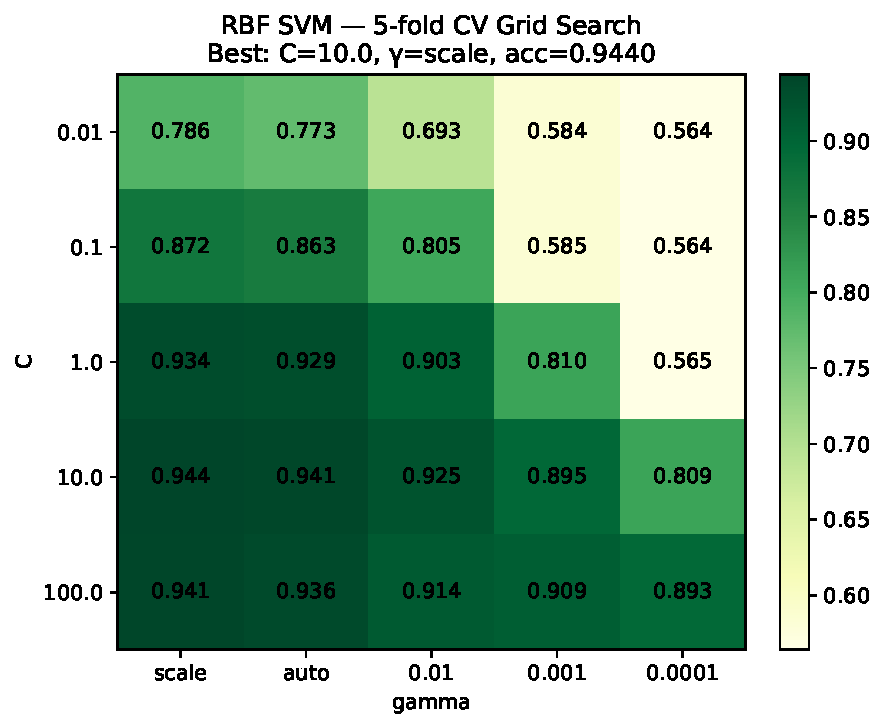
\includegraphics[width=0.65\textwidth]{results/eval_figures/eval_svm_grid.pdf}
    \caption{5-fold CV accuracy heatmap over $(C, \gamma)$ for RBF Kernel SVM on Trial~1.}
    \label{fig:svm_grid}
\end{figure}

\noindent \textbf{\textit{Analysis:}} Best configuration: $C\!=\!10$, $\gamma\!=\!\texttt{scale}$ (94.40\%). The \texttt{scale} setting computes $\gamma = 1/(d \cdot \mathrm{Var}(X))$, which automatically adapts to the feature dimensionality and spread — this outperforms all hand-tuned $\gamma$ values, demonstrating that data-driven parameter calibration is more robust than manual selection. Accuracy saturates for $C \geq 10$: beyond this point, the margin is already narrow enough to correctly classify most training samples, and further increasing $C$ only risks overfitting to outliers without improving generalization.

\subsubsection{Effect of PCA Variance Ratio}
PCA projects onto top eigenvectors. Too few components lose signal; too many preserve noise. We sweep 0.70--0.99 for LR and SVM.

\begin{figure}[H]
    \centering
    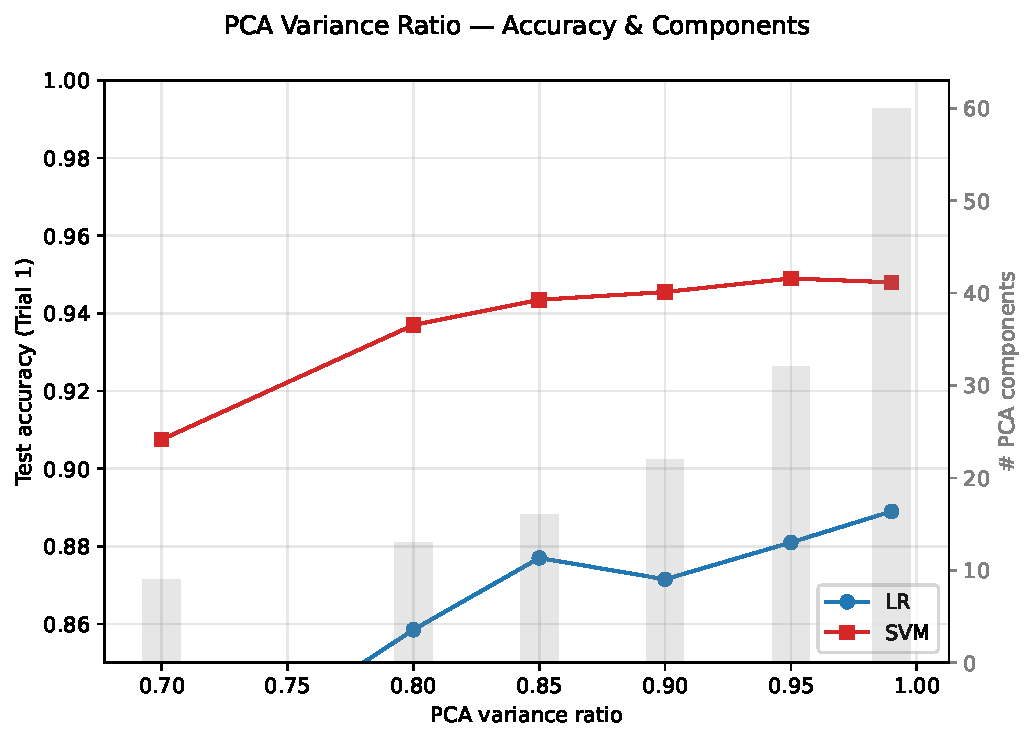
\includegraphics[width=0.82\textwidth]{results/eval_figures/eval_pca_variance.pdf}
    \caption{Effect of PCA variance ratio on test accuracy and number of retained components (Trial~1).}
    \label{fig:pca_var}
\end{figure}

\noindent \textbf{\textit{Analysis:}} SVM peaks at \textbf{0.95} ($\approx$32 dimensions). Beyond this, the additional principal components capture low-variance directions that are dominated by pixel noise; in the RBF kernel's distance computation, these noisy dimensions inflate $\|\mathbf{x}-\mathbf{x}'\|^2$ and degrade the kernel's discriminative power. LR, by contrast, improves monotonically to 0.99 ($\approx$60 dimensions): a linear classifier benefits from any feature with non-zero signal-to-noise ratio, since its $\mathbf{w}^\top\mathbf{x}$ projection can learn to down-weight noisy components via regularization. This opposite behavior motivates per-model PCA settings: 0.95 for SVM, 0.99 for LR.

\subsubsection{Linear PCA vs Kernel PCA}
Kernel PCA applies PCA in an implicit high-dimensional space. We compare Linear PCA against seven Kernel PCA variants across 10--160 dimensions.

\begin{figure}[H]
    \centering
    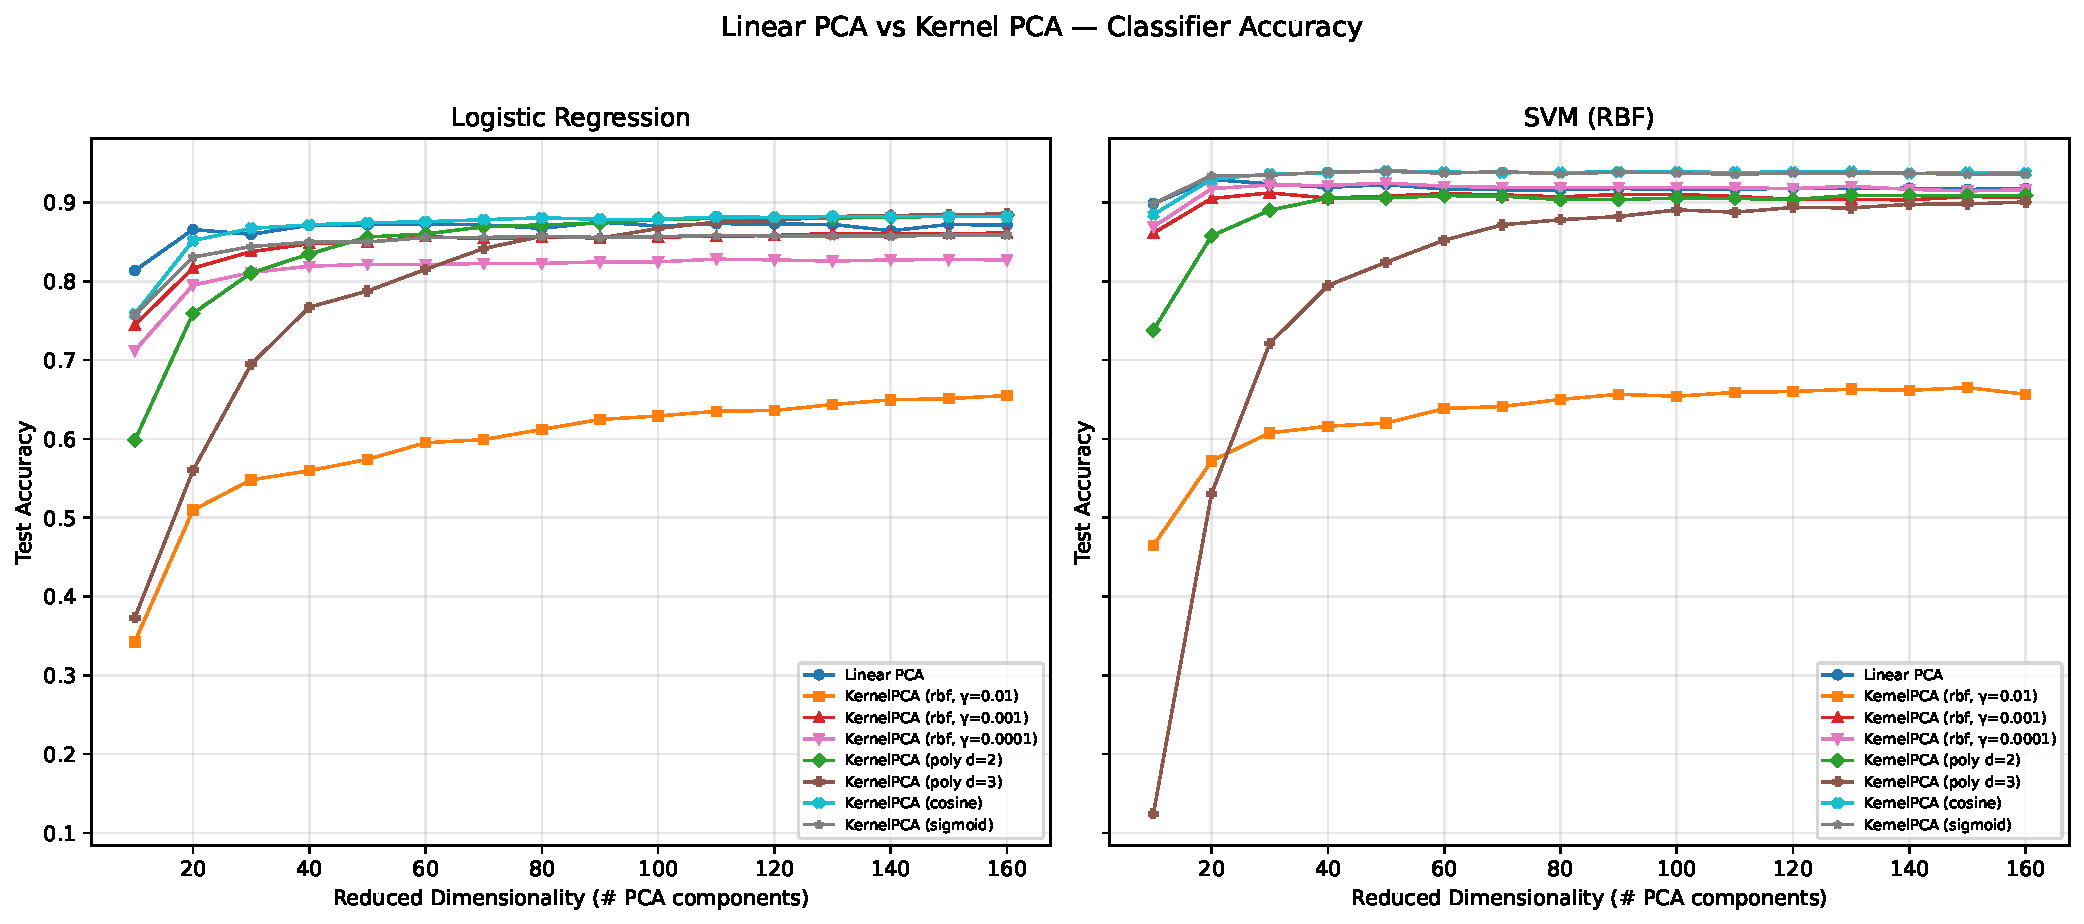
\includegraphics[width=\textwidth]{results/eval_figures/eval_kernel_pca.pdf}
    \caption{Linear PCA vs Kernel PCA — test accuracy across reduced dimensionalities on Trial~1.}
    \label{fig:kernel_pca}
\end{figure}

\noindent \textbf{\textit{Analysis:}} \textbf{Linear PCA} matches or outperforms all Kernel PCA variants for both classifiers. This indicates that the dominant variance structure of handwritten digit images lies along linear directions in pixel space — the digit manifold, while high-dimensional, is well-approximated by a linear subspace. Kernel PCA with small RBF $\gamma$ (0.01) consistently underperforms because an overly narrow kernel makes distant points appear equally dissimilar, collapsing the eigenspectrum. Given that Linear PCA is also computationally cheaper (no $N \times N$ kernel matrix), there is no justification for using Kernel PCA on this dataset.

\subsubsection{Summary}

The hyperparameter experiments reveal several consistent patterns. First, the \textbf{RBF kernel} is the optimal SVM choice — its infinite-dimensional mapping provides the flexibility for 10-class separation, while Linear and Sigmoid are limited by their hypothesis spaces. Second, the optimal point ($C\!=\!10$, $\gamma\!=\!\texttt{scale}$) balances expressiveness against overfitting; the data-adaptive \texttt{scale} setting proves more reliable than hand-tuned values. Third, PCA has \textbf{opposite effects} on SVM and LR: SVM favors aggressive reduction (0.95, $\sim$32 dims) because the RBF kernel is sensitive to noisy dimensions, while LR prefers retaining more features (0.99, $\sim$60 dims) as $L_2$ regularization can down-weight noise. Fourth, \textbf{Kernel PCA offers no advantage} — the digit manifold is well-approximated by a linear subspace. Finally, the \textbf{9--145$\times$ speed gap} necessitates library implementations for systematic exploration, though our from-scratch code achieves comparable or superior accuracy.

\section{Conclusion}

We implemented and evaluated seven classifiers on a 4000-sample MNIST subset. Key conclusions:

\begin{enumerate}
    \item \textbf{CNN achieves the best accuracy} (98.10\% base, 92.33\% challenge) with strongest robustness. Its convolutional layers exploit spatial locality and translation invariance, learning hierarchical features (edges $\to$ strokes $\to$ parts) that generalize across writing styles. This confirms that \emph{inductive bias aligned with data structure} is the most important factor.

    \item \textbf{Kernel SVM is the strongest traditional model} (94.80\%, lowest variance 0.0010). The RBF kernel constructs non-linear boundaries in high-dimensional space, and the max-margin objective provides inherent regularization — representing the upper bound for non-deep methods.

    \item \textbf{Preprocessing is model-dependent.} Image-domain filtering improves all vector-based models, but PCA helps SVM/LR while \emph{hurting} CNN, XGBoost, and RF, which benefit from the full 784-dimensional space.

    \item \textbf{Linear PCA suffices.} Seven Kernel PCA variants were tested; none outperformed standard PCA. The digit manifold is well-approximated by a linear subspace.

    \item \textbf{Per-model tuning is essential.} SVM and LR have opposite PCA preferences (0.95 vs 0.99); kernel choice drastically affects SVM (RBF: 94.4\% vs Sigmoid: $<$80\%); the grid search reveals a sharp optimum at $C\!=\!10$, $\gamma\!=\!\texttt{scale}$.

    \item \textbf{From-scratch implementations} are 9--145$\times$ slower than sklearn but achieve comparable or superior accuracy, validating our algorithmic understanding while demonstrating the practical value of optimized backends.
\end{enumerate}

The path from 91.60\% (1-NN) to 98.10\% (CNN) involves not just model selection, but a careful interplay of preprocessing, dimensionality reduction, kernel choice, and regularization. Thoughtful tuning of traditional methods (SVM at 94.80\%) closes much of the gap; the remaining distance requires the spatial inductive bias that convolutional networks provide.

\newpage
\appendix
\section*{Appendix: Implementation Details}
\addcontentsline{toc}{section}{Appendix: Implementation Details}

Components are categorized as \textbf{From-Scratch (S)} (NumPy/SciPy) or \textbf{Library-Based (L)} (scikit-learn, PyTorch, XGBoost). All in-class models and core preprocessing are from scratch.

\begin{table}[H]
    \centering
    \renewcommand{\arraystretch}{1.1}
    \small
    \caption{Component implementation and dependencies}
    \label{tab:impl_source}
    \begin{tabular}{lll}
        \toprule
        \textbf{Component} & \textbf{Source (Lib)} & \textbf{Technical Notes} \\
        \midrule
        Pre-processing      & From-Scratch (\texttt{np})   & Median/Gaussian filters, sub-pixel shift, PCA \\
        1-NN                & From-Scratch (\texttt{np})   & Vectorized $\ell_2$ distance implementation \\
        Logistic Regression & From-Scratch (\texttt{np, sp}) & Multinomial softmax + $L_2$; L-BFGS-B optimizer \\
        Kernel SVM          & From-Scratch (\texttt{np})   & Simplified SMO algorithm; One-vs-Rest; RBF \\
        Random Forest       & \textit{scikit-learn} (L)    & 500-tree \texttt{RandomForestClassifier} \\
        MLP                 & \textit{scikit-learn} (L)    & \texttt{MLPClassifier}; Arch: (512, 256, 128) \\
        CNN                 & \textit{PyTorch} (L)         & LeNet-style: 2$\times$Conv-BN-ReLU + Dropout \\
        XGBoost             & \textit{XGBoost} (L)         & Histogram-based tree; 150 rounds; $\eta=0.1$ \\
        \bottomrule
    \end{tabular}
\end{table}

Table~\ref{tab:model_config} summarizes the final hyperparameters, determined through the analyses in Section~3.3.

\begin{table}[H]
    \centering
    \renewcommand{\arraystretch}{1.15}
    \small
    \caption{Model configuration summary}
    \label{tab:model_config}
    \begin{tabular}{llll}
        \toprule
        \textbf{Model} & \textbf{Preprocessing} & \textbf{PCA} & \textbf{Key Hyperparameters} \\
        \midrule
        1-NN                & \texttt{noprocess}    & —               & $k = 1$ \\
        Logistic Regression & \texttt{wholeprocess} & 0.99            & $C = 1.0$; \texttt{max\_iter} = 300 \\
        Kernel SVM          & \texttt{wholeprocess} & 0.95            & $C = 10$; $\gamma = \texttt{scale}$ \\
        Random Forest       & \texttt{noPCA}        & —               & 500 trees; \texttt{max\_features} = $\sqrt{D}$ \\
        XGBoost             & \texttt{noPCA}        & —               & 150 rounds; $\eta = 0.1$; depth = 6 \\
        MLP                 & \texttt{wholeprocess} & 0.95            & Arch: (512, 256, 128); \texttt{lr} = 0.005 \\
        CNN                 & \texttt{noPCA}        & —               & 50 epochs; \texttt{lr} = 0.001; batch = 64 \\
        \bottomrule
    \end{tabular}
\end{table}

Environment dependencies (Table~\ref{tab:requirements}):

\begin{table}[H]
    \centering
    \renewcommand{\arraystretch}{1.1}
    \small
    \caption{Project environment dependencies (\texttt{requirements.txt})}
    \label{tab:requirements}
    \begin{tabular}{llp{7.5cm}}
        \toprule
        \textbf{Package} & \textbf{Category} & \textbf{Primary Role} \\
        \midrule
        \texttt{numpy}        & Numerical & Linear algebra for scratch models and pre-processing \\
        \texttt{scipy}        & Optimization & Scientific primitives (L-BFGS-B) for LR model \\
        \texttt{scikit-learn} & ML Library   & Ensemble models, MLP, and evaluation metrics \\
        \texttt{xgboost}      & Gradient Boosting & High-performance gradient boosting framework \\
        \texttt{torch}        & Deep Learning & CNN definition, GPU acceleration, and training loop \\
        \texttt{joblib}       & Serialization & Model persistence (Save/Load) \\
        \texttt{matplotlib}   & Visualization & Result plotting and image export to \texttt{results/images/} \\
        \bottomrule
    \end{tabular}
\end{table}

\newpage
\section*{Appendix: Confusion Matrices}
\addcontentsline{toc}{section}{Appendix: Confusion Matrices}

The following figures present per-model confusion matrices for both experimental trials. Each figure shows Trial~1 (left) and Trial~2 (right) side by side.

\subsection*{B.1\quad Base Test Set}

\begin{figure}[H]
    \centering
    \begin{subfigure}{0.48\textwidth}
        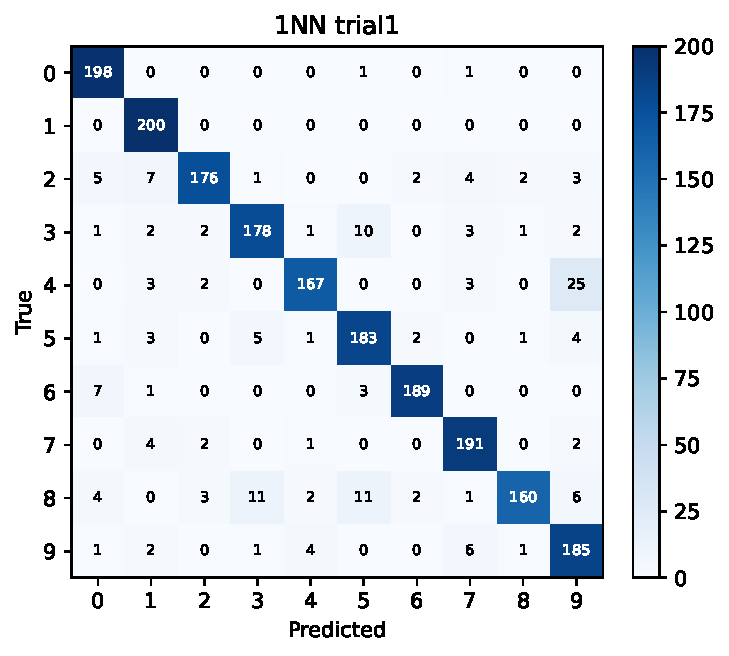
\includegraphics[width=\textwidth]{results/images/1NN_trial1.pdf}
        \caption{Trial 1}
    \end{subfigure}\hfill
    \begin{subfigure}{0.48\textwidth}
        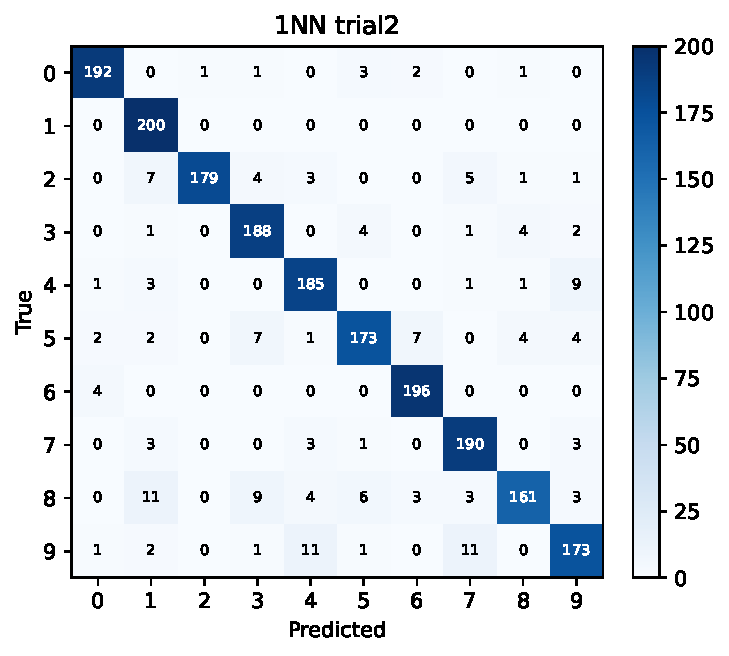
\includegraphics[width=\textwidth]{results/images/1NN_trial2.pdf}
        \caption{Trial 2}
    \end{subfigure}
    \caption{1-NN (Baseline) — Base test set.}
\end{figure}

\begin{figure}[H]
    \centering
    \begin{subfigure}{0.48\textwidth}
        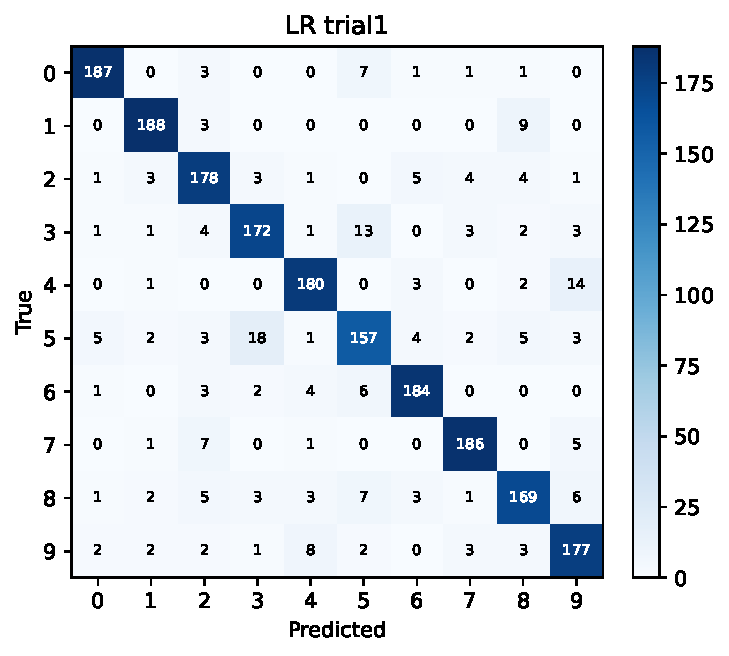
\includegraphics[width=\textwidth]{results/images/LR_trial1.pdf}
        \caption{Trial 1}
    \end{subfigure}\hfill
    \begin{subfigure}{0.48\textwidth}
        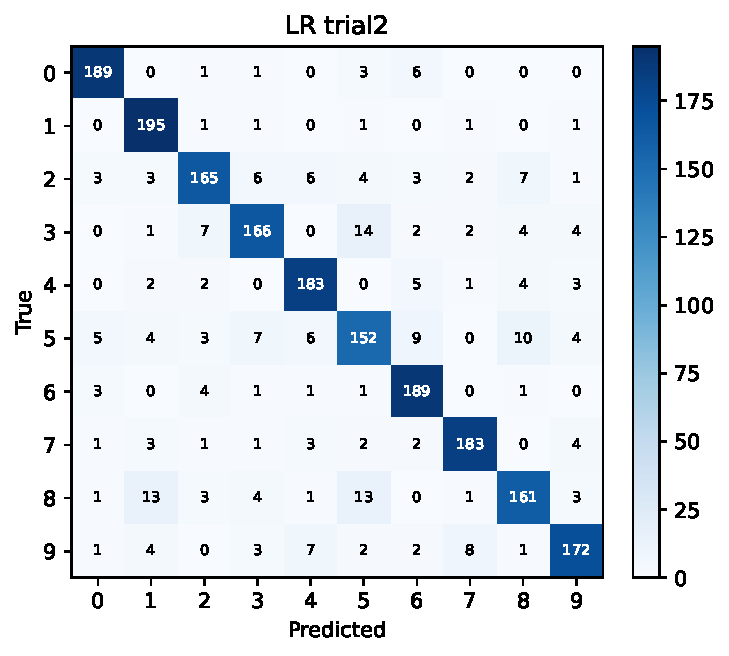
\includegraphics[width=\textwidth]{results/images/LR_trial2.pdf}
        \caption{Trial 2}
    \end{subfigure}
    \caption{Logistic Regression — Base test set.}
\end{figure}

\begin{figure}[H]
    \centering
    \begin{subfigure}{0.48\textwidth}
        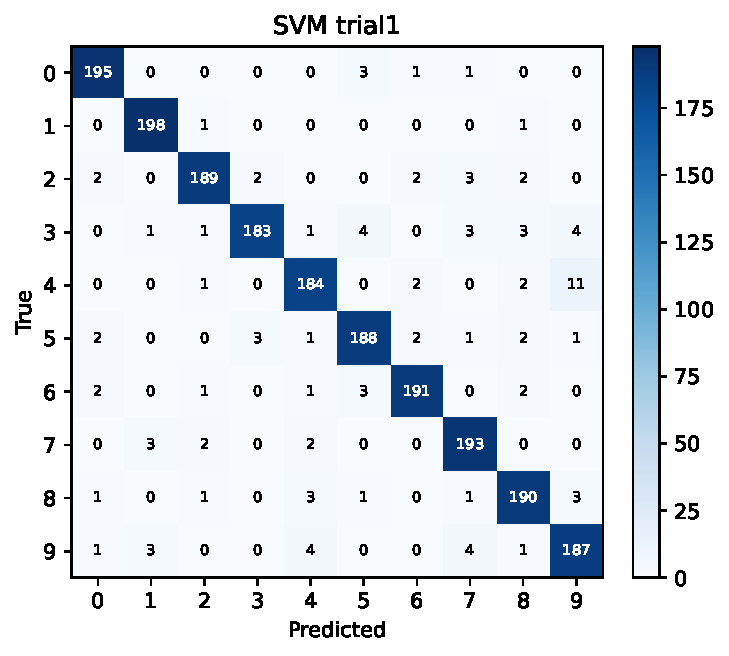
\includegraphics[width=\textwidth]{results/images/SVM_trial1.pdf}
        \caption{Trial 1}
    \end{subfigure}\hfill
    \begin{subfigure}{0.48\textwidth}
        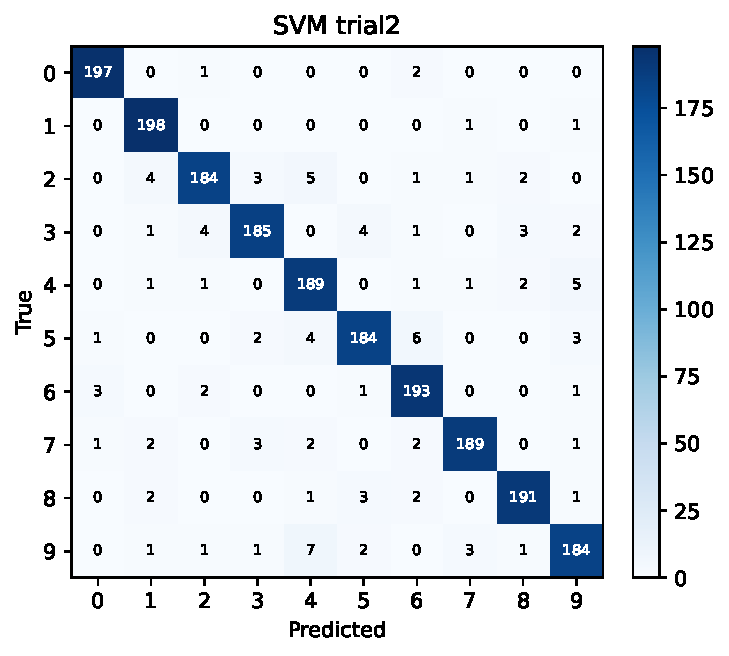
\includegraphics[width=\textwidth]{results/images/SVM_trial2.pdf}
        \caption{Trial 2}
    \end{subfigure}
    \caption{Kernel SVM — Base test set.}
\end{figure}

\begin{figure}[H]
    \centering
    \begin{subfigure}{0.48\textwidth}
        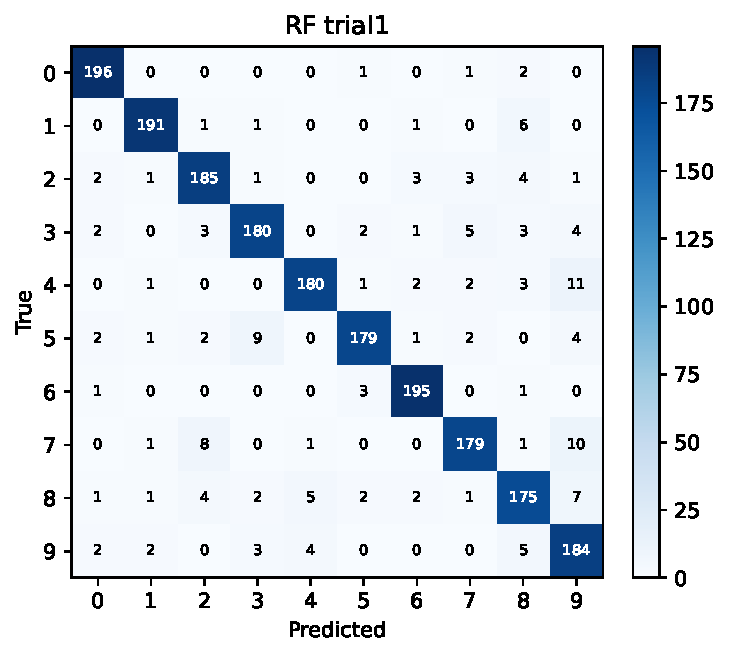
\includegraphics[width=\textwidth]{results/images/RF_trial1.pdf}
        \caption{Trial 1}
    \end{subfigure}\hfill
    \begin{subfigure}{0.48\textwidth}
        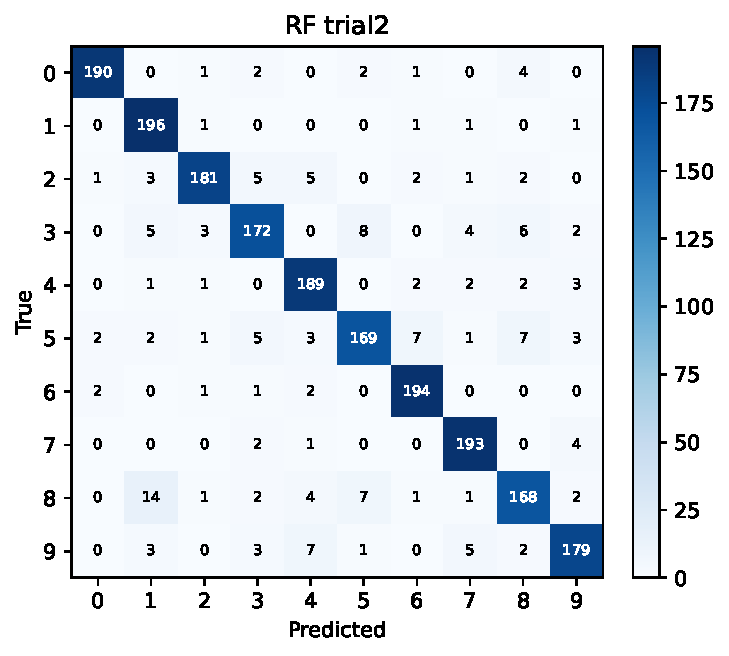
\includegraphics[width=\textwidth]{results/images/RF_trial2.pdf}
        \caption{Trial 2}
    \end{subfigure}
    \caption{Random Forest — Base test set.}
\end{figure}

\begin{figure}[H]
    \centering
    \begin{subfigure}{0.48\textwidth}
        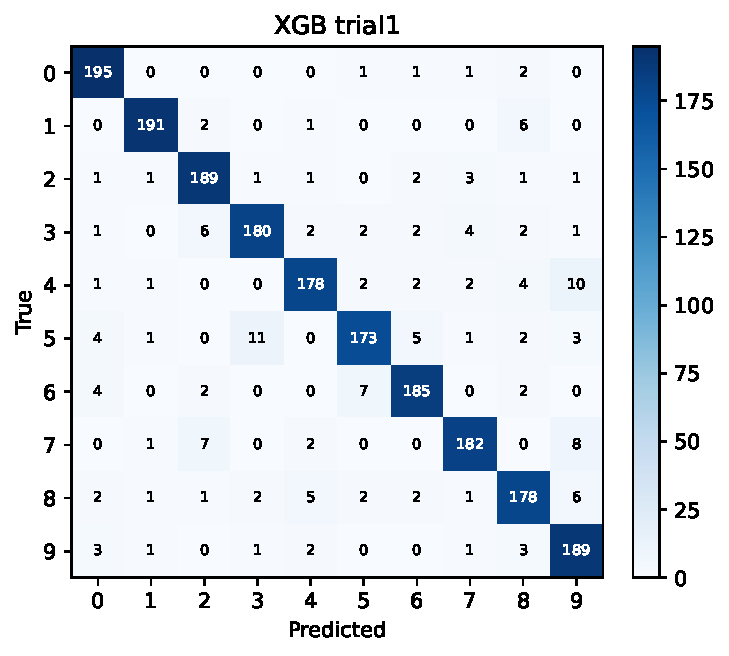
\includegraphics[width=\textwidth]{results/images/XGB_trial1.pdf}
        \caption{Trial 1}
    \end{subfigure}\hfill
    \begin{subfigure}{0.48\textwidth}
        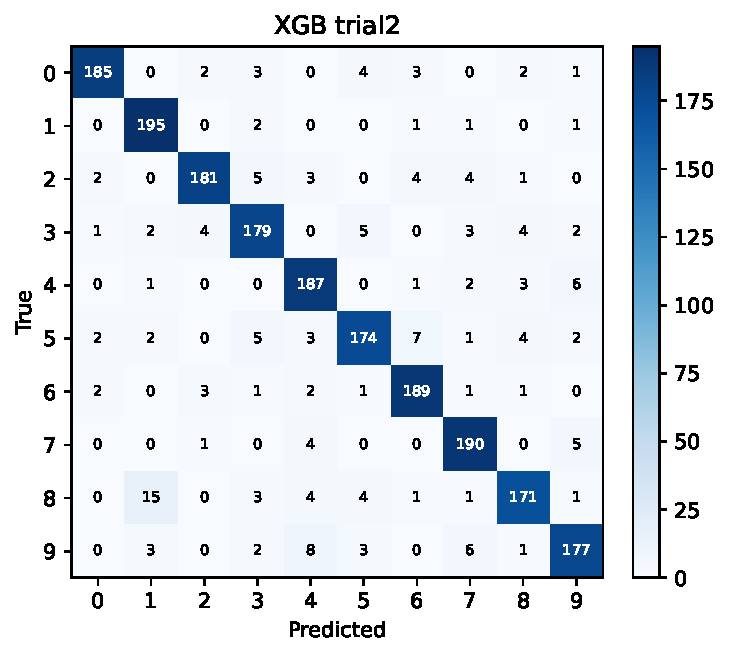
\includegraphics[width=\textwidth]{results/images/XGB_trial2.pdf}
        \caption{Trial 2}
    \end{subfigure}
    \caption{XGBoost — Base test set.}
\end{figure}

\begin{figure}[H]
    \centering
    \begin{subfigure}{0.48\textwidth}
        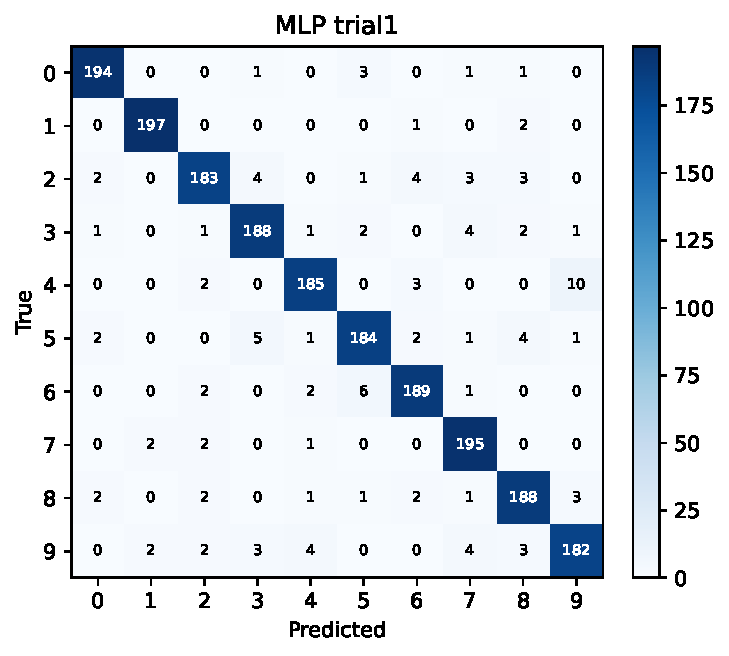
\includegraphics[width=\textwidth]{results/images/MLP_trial1.pdf}
        \caption{Trial 1}
    \end{subfigure}\hfill
    \begin{subfigure}{0.48\textwidth}
        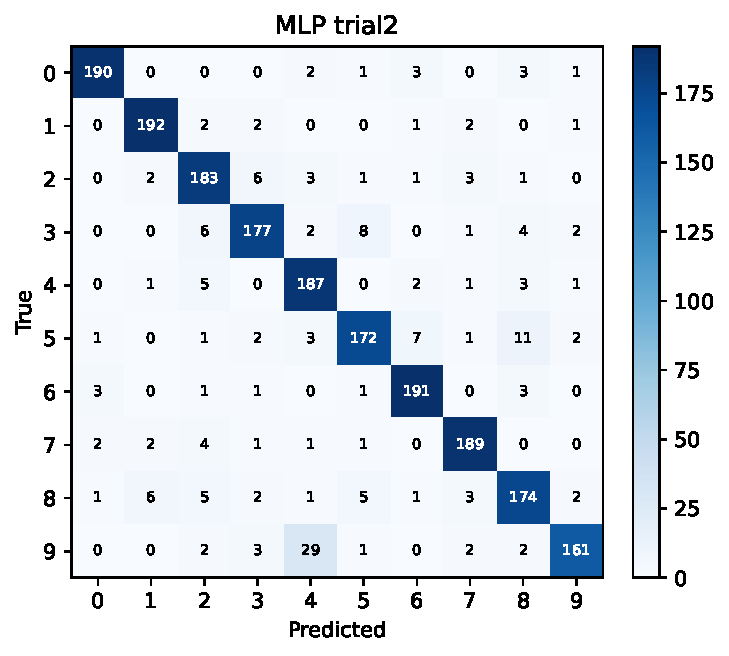
\includegraphics[width=\textwidth]{results/images/MLP_trial2.pdf}
        \caption{Trial 2}
    \end{subfigure}
    \caption{MLP — Base test set.}
\end{figure}

\begin{figure}[H]
    \centering
    \begin{subfigure}{0.48\textwidth}
        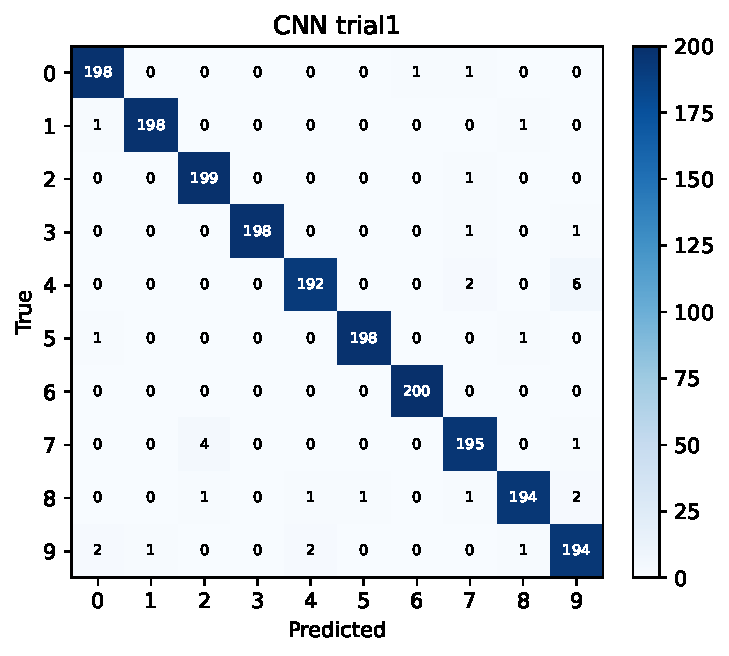
\includegraphics[width=\textwidth]{results/images/CNN_trial1.pdf}
        \caption{Trial 1}
    \end{subfigure}\hfill
    \begin{subfigure}{0.48\textwidth}
        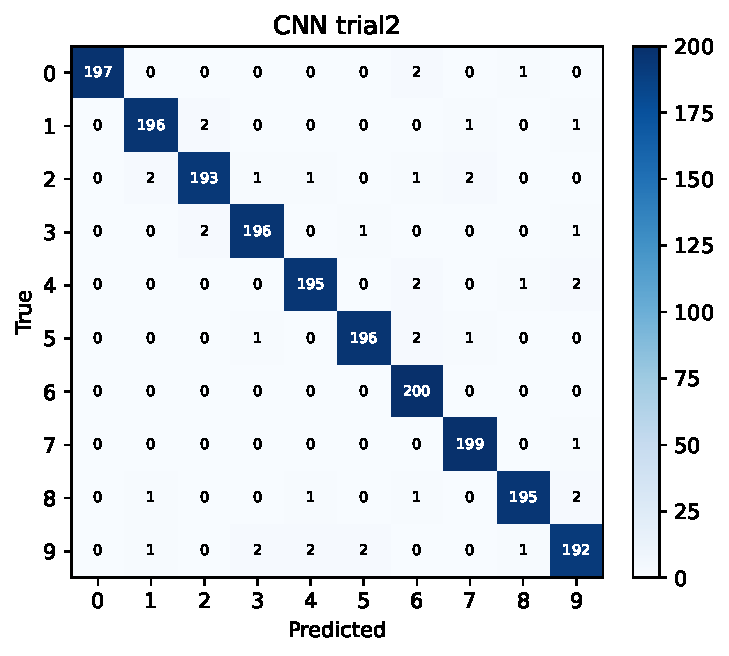
\includegraphics[width=\textwidth]{results/images/CNN_trial2.pdf}
        \caption{Trial 2}
    \end{subfigure}
    \caption{CNN — Base test set.}
\end{figure}

\subsection*{B.2\quad Challenge Dataset}

\begin{figure}[H]
    \centering
    \begin{subfigure}{0.48\textwidth}
        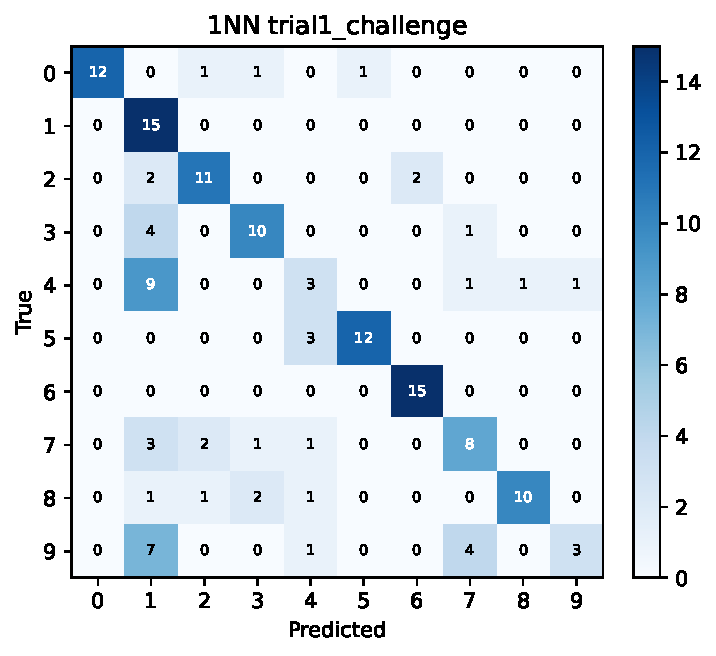
\includegraphics[width=\textwidth]{results/images/1NN_trial1_challenge.pdf}
        \caption{Trial 1}
    \end{subfigure}\hfill
    \begin{subfigure}{0.48\textwidth}
        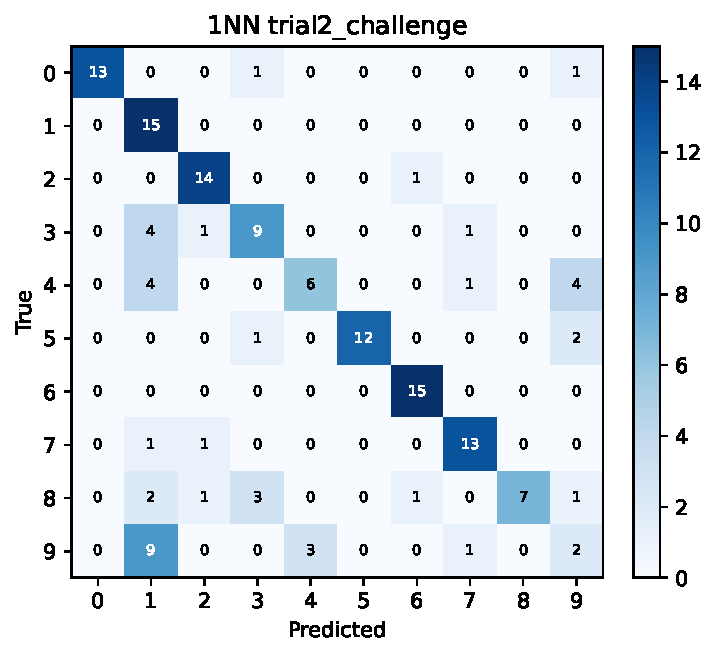
\includegraphics[width=\textwidth]{results/images/1NN_trial2_challenge.pdf}
        \caption{Trial 2}
    \end{subfigure}
    \caption{1-NN (Baseline) — Challenge dataset.}
\end{figure}

\begin{figure}[H]
    \centering
    \begin{subfigure}{0.48\textwidth}
        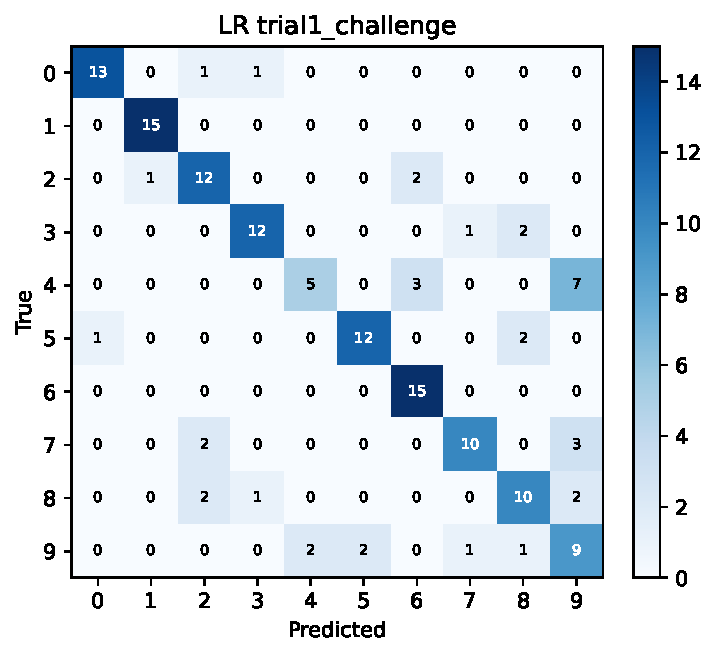
\includegraphics[width=\textwidth]{results/images/LR_trial1_challenge.pdf}
        \caption{Trial 1}
    \end{subfigure}\hfill
    \begin{subfigure}{0.48\textwidth}
        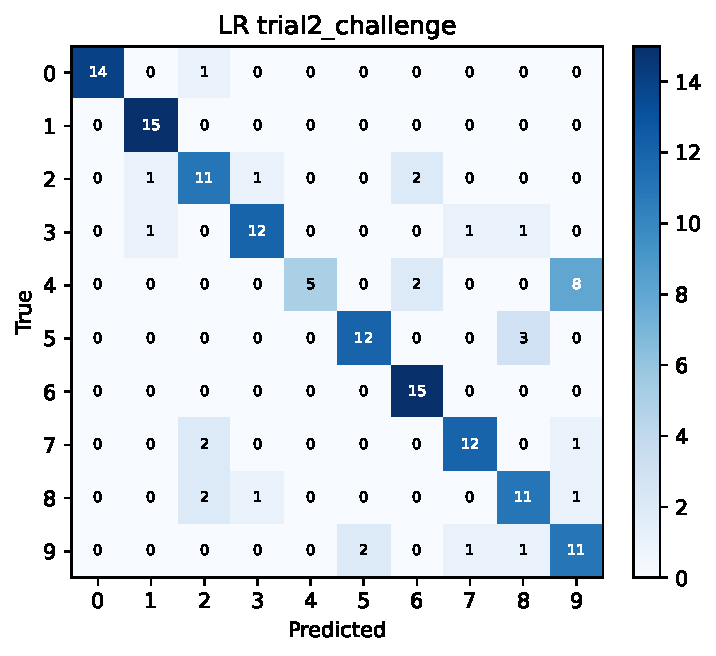
\includegraphics[width=\textwidth]{results/images/LR_trial2_challenge.pdf}
        \caption{Trial 2}
    \end{subfigure}
    \caption{Logistic Regression — Challenge dataset.}
\end{figure}

\begin{figure}[H]
    \centering
    \begin{subfigure}{0.48\textwidth}
        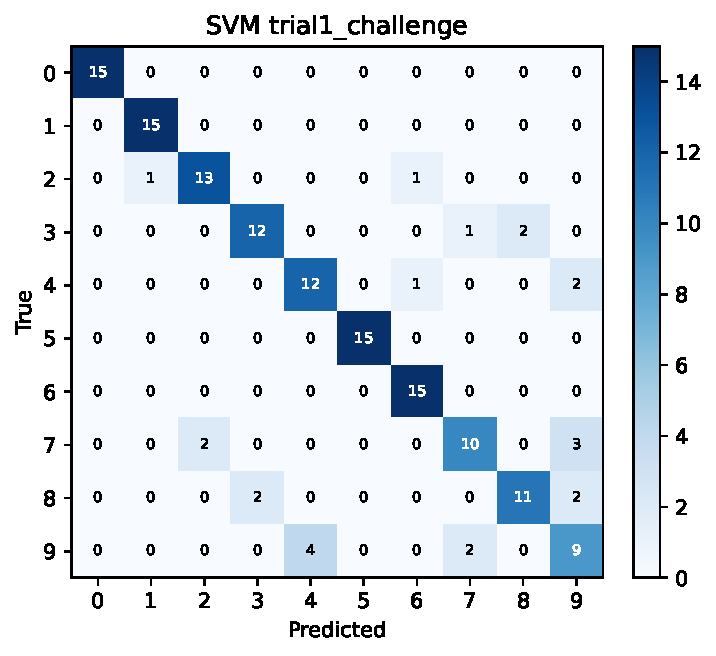
\includegraphics[width=\textwidth]{results/images/SVM_trial1_challenge.pdf}
        \caption{Trial 1}
    \end{subfigure}\hfill
    \begin{subfigure}{0.48\textwidth}
        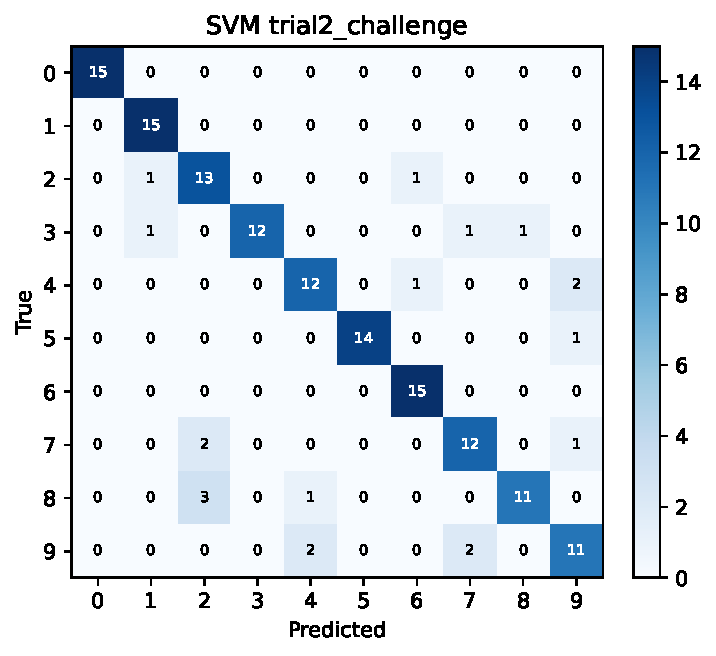
\includegraphics[width=\textwidth]{results/images/SVM_trial2_challenge.pdf}
        \caption{Trial 2}
    \end{subfigure}
    \caption{Kernel SVM — Challenge dataset.}
\end{figure}

\begin{figure}[H]
    \centering
    \begin{subfigure}{0.48\textwidth}
        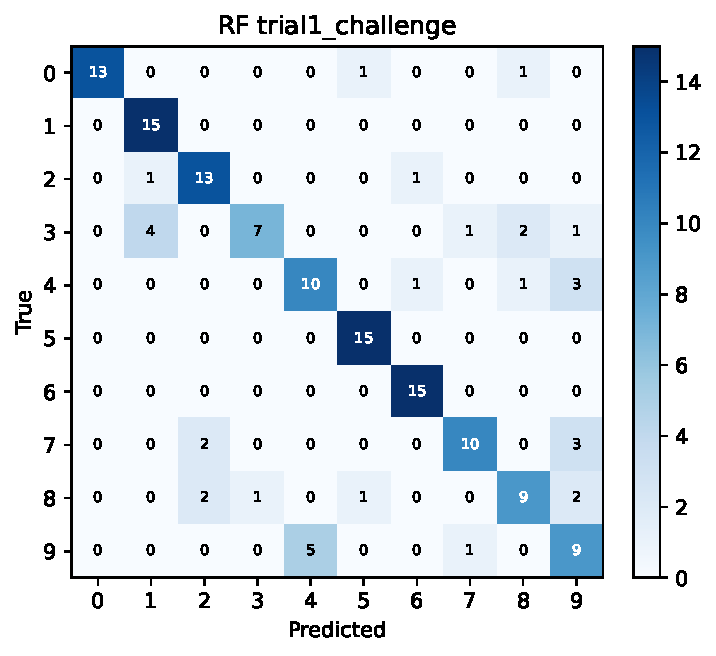
\includegraphics[width=\textwidth]{results/images/RF_trial1_challenge.pdf}
        \caption{Trial 1}
    \end{subfigure}\hfill
    \begin{subfigure}{0.48\textwidth}
        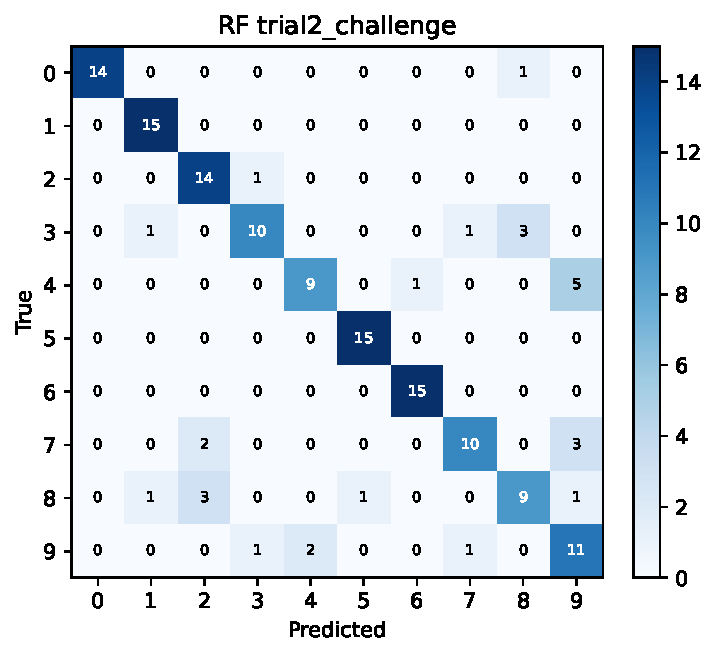
\includegraphics[width=\textwidth]{results/images/RF_trial2_challenge.pdf}
        \caption{Trial 2}
    \end{subfigure}
    \caption{Random Forest — Challenge dataset.}
\end{figure}

\begin{figure}[H]
    \centering
    \begin{subfigure}{0.48\textwidth}
        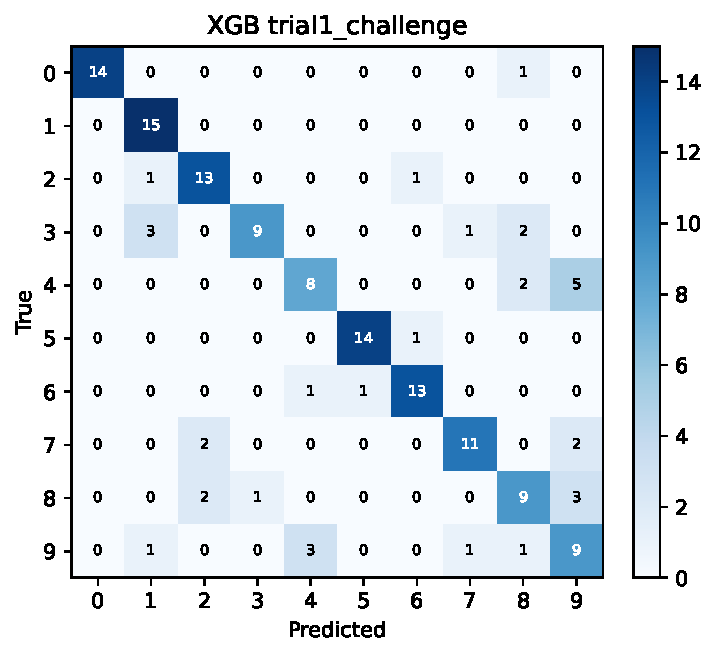
\includegraphics[width=\textwidth]{results/images/XGB_trial1_challenge.pdf}
        \caption{Trial 1}
    \end{subfigure}\hfill
    \begin{subfigure}{0.48\textwidth}
        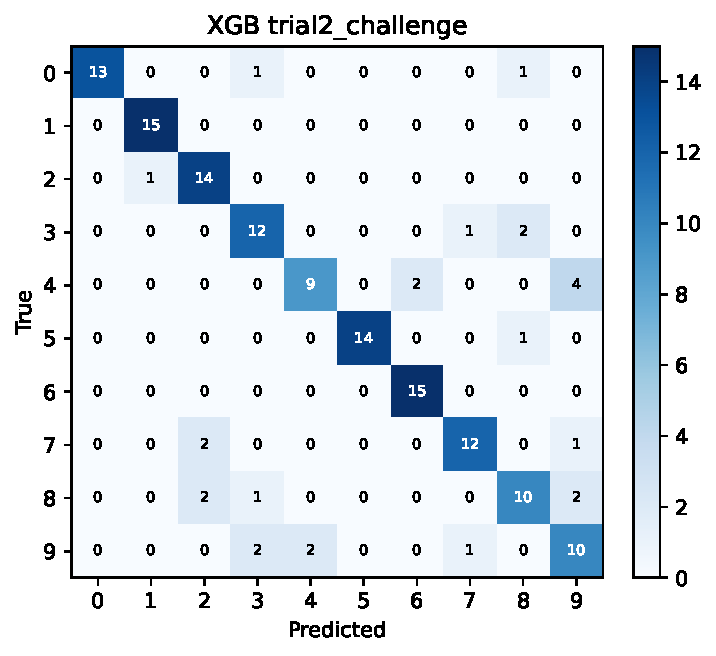
\includegraphics[width=\textwidth]{results/images/XGB_trial2_challenge.pdf}
        \caption{Trial 2}
    \end{subfigure}
    \caption{XGBoost — Challenge dataset.}
\end{figure}

\begin{figure}[H]
    \centering
    \begin{subfigure}{0.48\textwidth}
        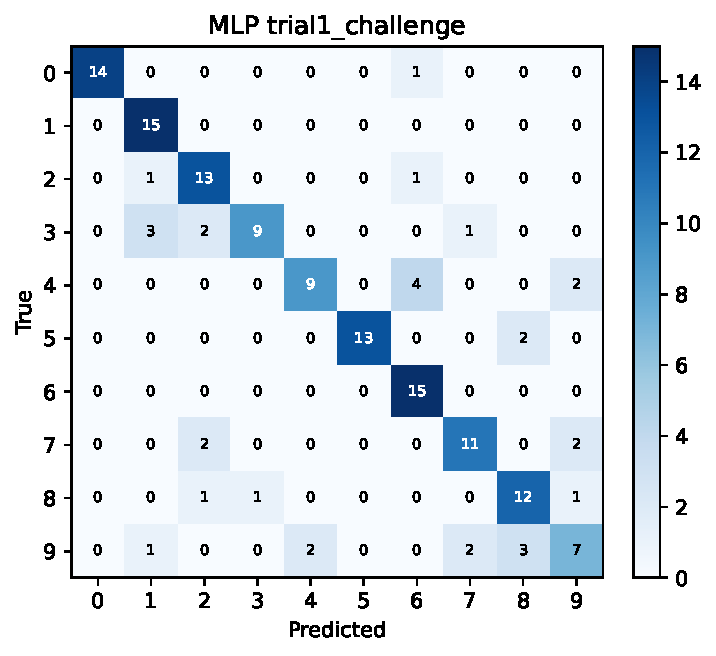
\includegraphics[width=\textwidth]{results/images/MLP_trial1_challenge.pdf}
        \caption{Trial 1}
    \end{subfigure}\hfill
    \begin{subfigure}{0.48\textwidth}
        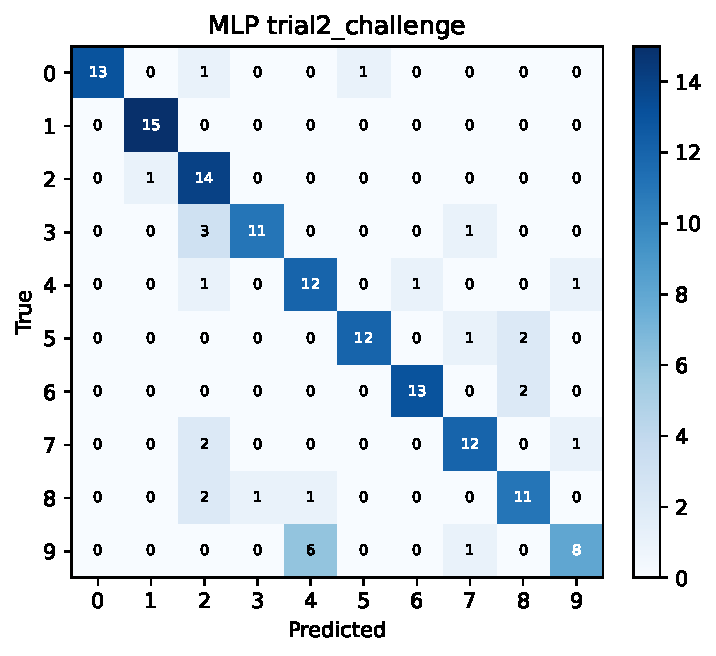
\includegraphics[width=\textwidth]{results/images/MLP_trial2_challenge.pdf}
        \caption{Trial 2}
    \end{subfigure}
    \caption{MLP — Challenge dataset.}
\end{figure}

\begin{figure}[H]
    \centering
    \begin{subfigure}{0.48\textwidth}
        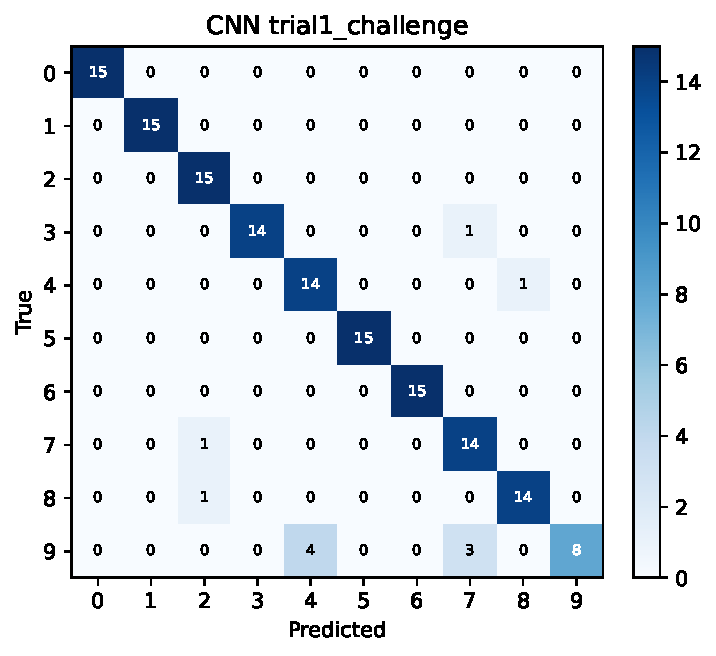
\includegraphics[width=\textwidth]{results/images/CNN_trial1_challenge.pdf}
        \caption{Trial 1}
    \end{subfigure}\hfill
    \begin{subfigure}{0.48\textwidth}
        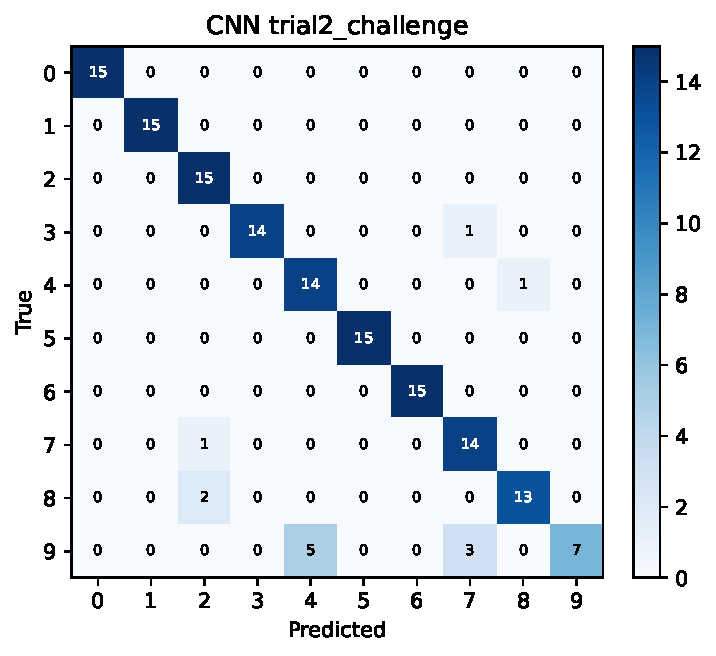
\includegraphics[width=\textwidth]{results/images/CNN_trial2_challenge.pdf}
        \caption{Trial 2}
    \end{subfigure}
    \caption{CNN — Challenge dataset.}
\end{figure}

\newpage
\section*{Appendix: Quick-Start Guide}
\addcontentsline{toc}{section}{Appendix: Quick-Start Guide}

The project root is structured as follows (non-essential files omitted):

\begin{verbatim}
.
├── main.py                  # unified entry point
├── Makefile                 # make targets (see below)
├── requirements.txt         # Python dependencies
├── check_env.py             # environment & data verifier
├── pipeline/                # models and preprocessing
│   ├── preprocess.py        #   preprocessing pipeline
│   ├── OneNN.py             #   1-NN (from scratch)
│   ├── LogisticRegression.py#   Softmax LR (from scratch)
│   ├── KernelSVM.py         #   RBF SVM (from scratch)
│   ├── RandomForest.py      #   sklearn RandomForest
│   ├── XGBoost.py           #   XGBoost wrapper
│   ├── MLP.py               #   sklearn MLP
│   └── CNN.py               #   PyTorch LeNet-style CNN
├── evaluation/              # hyperparameter analysis scripts
├── utils/                   # I/O helpers (data, model, results)
├── data/raw/                # MNIST base + challenge data
├── data/trained-model/      # saved model checkpoints
└── results/                 # outputs (JSON, images, eval figures)
\end{verbatim}

\noindent All operations are invoked via \texttt{make} from the project root:

\begin{table}[H]
    \centering
    \renewcommand{\arraystretch}{1.15}
    \small
    \begin{tabular}{lp{9cm}}
        \toprule
        \textbf{Command} & \textbf{Description} \\
        \midrule
        \texttt{make all}       & Run the full pipeline end-to-end: build $\to$ checkenv $\to$ train $\to$ base $\to$ challenge $\to$ eval. \\
        \texttt{make build}     & Install all Python dependencies from \texttt{requirements.txt}. \\
        \texttt{make checkenv}  & Print the Python version, then run \texttt{check\_env.py} to verify that all packages and data files are present. \\
        \texttt{make train}     & Train all models on both trials and save checkpoints to \texttt{data/trained-model/}. \\
        \texttt{make base}      & Evaluate all models on the base test set (loads saved models; trains if missing). Outputs confusion matrices to \texttt{results/images/}. \\
        \texttt{make eval}      & Run the four hyperparameter sensitivity analysis scripts in \texttt{evaluation/}. Outputs figures to \texttt{results/eval\_figures/}. \\
        \texttt{make challenge} & Evaluate all models on the challenge dataset. \\
        \texttt{make clean}     & Remove saved models and Python caches. \\
        \bottomrule
    \end{tabular}
    \caption{Available \texttt{make} targets.}
\end{table}

\noindent \textbf{Recommended workflow:}
\begin{verbatim}
make all          # run everything end-to-end
\end{verbatim}

\noindent Or step by step:
\begin{verbatim}
make build        # 1. install dependencies
make checkenv     # 2. verify environment
make train        # 3. train all models
make base         # 4. evaluate on base test set
make challenge    # 5. evaluate on challenge set
make eval         # 6. generate analysis figures
\end{verbatim}

\end{document}